\chapter{Machine learning e visualizzazioni vaghe}
\label{cap:visualizzazioni-vaghe}

\section{Machine learning in ambito medico }

Negli ultimi anni, l'IA ha conosciuto uno sviluppo significativo, rendendo possibile immaginare un futuro in cui diagnosi errate e trattamenti sintomatici saranno superati. La gestione e l'analisi delle enormi quantità di dati generate dalle immagini mediche e dai test diagnostici consentono all'IA di sviluppare applicazioni sofisticate, inaugurando un'era di medicina elettronica.\\
Nonostante alcuni algoritmi siano in grado di eguagliare e talvolta superare i clinici in varie attività, l'IA non è ancora integrata completamente nella pratica medica quotidiana. Questo ritardo è dovuto a una serie di sfide che devono essere affrontate prima di poter sfruttare appieno il potenziale dell'IA in medicina.\\

I sistemi di IA apprendono mediante un processo analogo a quello degli studenti di medicina, ovvero tramite analisi di dati, esecuzione di compiti pratici e apprendimento dagli errori. Dopo aver elaborato un numero sufficiente di dati e annotazioni, le prestazioni dell'algoritmo vengono valutate per verificarne l'accuratezza, simile agli esami per gli studenti di medicina. Questo processo di valutazione include l'utilizzo di dati di prova con risposte note per verificare la capacità dell'algoritmo di identificare correttamente le risposte. In base ai risultati, l'algoritmo può essere modificato, alimentato con ulteriori dati o implementato.\\

Molti algoritmi di IA possono apprendere dai dati, sia che si tratti di immagini mediche (come le scansioni MRI) sia di dati numerici (come la pressione sanguigna). Dopo aver elaborato questi dati, gli algoritmi sono in grado di fornire risultati probabilistici o classificazioni, come identificare un campione di tessuto come canceroso o stimare la probabilità di un coagulo arterioso. Le prestazioni degli algoritmi vengono poi confrontate con quelle dei medici per determinare se la diagnosi dell'IA è accurata e clinicamente rilevante.\\

Un esempio significativo di IA in ambito medico è l'algoritmo DLAD (Rilevamento Automatico basato su Apprendimento Profondo), sviluppato presso l'Università Nazionale di Seoul. Questo algoritmo analizza le radiografie del torace per rilevare crescite cellulari anomale, come i tumori. Nei test comparativi, DLAD ha dimostrato di superare 17 su 18 medici nella capacità di rilevamento delle anomalie.\\
Un altro esempio significativo di algoritmo IA nel settore medico è stato sviluppato nell'autunno del 2018 dai ricercatori di Google AI Healthcare. Questo algoritmo, denominato LYNA (Assistente dei Linfonodi), è stato progettato per identificare i tumori metastatici del cancro al seno dalle biopsie dei linfonodi. LYNA rappresenta un progresso significativo poiché è in grado di individuare aree sospette nei campioni di biopsia, una capacità che va oltre la percezione visiva umana. Nei test condotti su due diversi database, LYNA ha dimostrato un'accuratezza del 99\% nel classificare i campioni come cancerosi o non cancerosi. Inoltre, ha ridotto della metà il tempo medio di revisione delle diapositive quando utilizzato dai medici come supporto alla loro analisi tradizionale.\\
Altri algoritmi basati su immagini hanno mostrato abilità simili nel migliorare l'accuratezza diagnostica dei medici. Nel breve termine, questi algoritmi possono essere utilizzati per confermare diagnosi e spiegare più rapidamente i risultati ai pazienti senza compromettere l'accuratezza. A lungo termine, algoritmi approvati dalle autorità competenti potrebbero operare autonomamente, consentendo ai medici di concentrarsi su casi complessi che richiedono l'intervento umano.\\
Esempi come DLAD e LYNA dimostrano come gli algoritmi possano supportare i medici nella classificazione di campioni patologici, evidenziando caratteristiche delle immagini che necessitano di un'analisi più approfondita. Tuttavia, nonostante i benefici potenziali per pazienti e medici, l'integrazione clinica degli algoritmi IA è frenata da sfide burocratiche significative.\\

Recentemente è stato condotto un nuovo studio\footcite{womak:machine-learning-in-orthopedics} che esplora l'applicazione delle tecniche di machine learning (ML) in ambito ortopedico; il suo focus è esaminare articoli pubblicati negli ultimi vent'anni e farne una revisione.\\
In questo studio il machine learning è definito come lo studio di come gli algoritmi possono "imparare" relazioni complesse dai dati empirici, producendo modelli matematici che collegano numerose variabili a una variabile target di interesse. In medicina, questo significa poter prevedere, data una serie di immagini radiologiche, risultati di laboratorio o dati estratti da registri elettronici, etichette diagnostiche, livelli di risultato, valori di esami o opzioni di trattamento per aiutare i medici a prendere decisioni più accurate ed efficienti.\\

La revisione della letteratura è stata condotta eseguendo una ricerca sui database Medline e Scopus, includendo articoli che utilizzano tecniche di ML per il sistema muscoloscheletrico umano. Sono stati selezionati sei settori anatomici principali: colonna vertebrale, anca, ginocchio, caviglia, mano e piede, oltre a una procedura generale, l'artroplastica. Sono stati selezionati 70 articoli per una revisione approfondita del loro contenuto e codifica.\\
Gli articoli sono stati divisi in due categorie principali: tecniche di ML convenzionali e deep learning.
Tecniche di ML convenzionali:
\begin{itemize}
\item Decision Trees e Random Forests: Queste tecniche sono state utilizzate per classificare i soggetti con osteoartrite e per fornire interpretabilità clinica dei risultati.
\item Nearest Neighbors (NN): Utilizzate per varie applicazioni, tra cui la segmentazione delle immagini.
\item Regressione Lineare e Altre Tecniche Simili: Impiegate per modellare relazioni lineari tra variabili.
\item Support Vector Machines (SVM): Ampiamente usate per la classificazione e il rilevamento delle caratteristiche.
\item K-means Clustering e Altre Tecniche Simili: Utilizzate per raggruppare i dati in base a caratteristiche simili.
\item Altre Tecniche Discriminative: Come gradient boost machines e LDA.
\item Tecniche Generative: Come i modelli probabilistici, utilizzati per prevedere la progressione della scoliosi.
\end{itemize}


\subsection{Deep Learning}
Il deep learning, una sottocategoria del ML che utilizza reti neurali profonde, è particolarmente efficace per la gestione di grandi volumi di dati, come immagini mediche e dati sensoristici. Questo metodo è stato applicato a diverse aree dell'ortopedia, dimostrando un'elevata precisione in compiti come la segmentazione delle immagini e la classificazione delle patologie.\\
I risultati sono stati presentati anche visivamente, mostrando l'uso predominante delle tecniche di deep learning e SVM nei dati di imaging medico. Le analisi bibliometriche indicano un crescente interesse per l'applicazione del ML in ortopedia negli ultimi anni, con una tendenza verso l'uso di tecniche più avanzate e la collaborazione tra diversi gruppi di ricerca.\\
Gli autori hanno concluso che, sebbene il ML abbia dimostrato risultati promettenti in vari campi ortopedici, è necessaria una valutazione rigorosa e una validazione in contesti reali prima che possa essere ampiamente adottato nella pratica clinica. Attualmente, l'adozione del ML in ortopedia è ancora in una fase preliminare, con necessità di ulteriori studi e ricerche per consolidarne l'applicabilità e l'efficacia.


\subsection{Cosa ne pensano gli utenti nel 2024}
Secondo una recente indagine\footcite{womak:intelligenza-artificiale-e-medicina} dell'EngageMinds HUB, il Centro di ricerca dell'Università Cattolica, gli italiani ad oggi segnalano fiducia e timori verso l'uso dell'intelligenza artificiale in ambito medico.\\
Dal loro studio emerge che 6 italiani su 10 sono favorevoli all'uso dell'Intelligenza artificiale in ambito sanitario, di questi, l'88\% la userebbe per semplificare il linguaggio dei referti, l'86\% come supporto al medico per effettuare una diagnosi e l'80\% come aiuto per stabilire una terapia farmacologica adeguata, mentre quasi 6 italiani su 10 la utilizzerebbero come strumento per un'autoanalisi.\\
Di opinione meno positiva sono 7 italiani su 10 secondo i quali l'AI potrà causare una perdita della relazione e del contatto diretto con il medico.\\

Tra le principali opportunità che l'uso delle tecnologie digitali potranno portare, poco meno di 8 italiani su 10 (78\%) riferiscono che esse porteranno ad una maggiore accessibilità nell'accesso e nell'uso dei servizi, una riduzione dello spreco di carta e un maggior coinvolgimento del paziente grazie ad una maggiore accessibilità al proprio fascicolo sanitario. Il 74\% crede che le AI potranno ridurre i costi a lungo termine; poco meno di 7 su 10 ritengono che possa esserci un miglioramento nei monitoraggi tramite devices (68\%), mentre poco più di 6 su 10 si aspetta che le AI possano migliorare le diagnosi (63\%). Il 68\% degli italiani ritiene che l'uso di tecnologie digitali possano migliorare il monitoraggio da
remoto.\\

Un ulteriore rischio che gli italiani percepiscono è legato ai dati sensibili: per il 63\% l'uso dell'Intelligenza Artificiale potrà causare delle problematiche legate alla gestione della privacy, mentre per il 60\% legate alla diffusione di dati sensibili.


\section{Visualizzazioni vaghe}
Le visualizzazioni vaghe, o "fuzzy visualizations", sono un concetto importante in data science che aiuta a gestire l'incertezza e la variabilità nei dati. Quando si tratta di analisi dei dati, spesso ci troviamo a dover affrontare informazioni che contengono errori, rumore o incertezze intrinseche. Le visualizzazioni vaghe sono progettate per rappresentare queste incertezze in modo che gli utenti possano avere una comprensione più completa e affidabile delle informazioni presentate.\\

Uno dei metodi più comuni utilizzati nelle visualizzazioni vaghe è l'impiego degli intervalli di confidenza. Questi intervalli indicano la gamma di valori entro cui si prevede che un parametro si trovi con una certa probabilità. Ad esempio, in un grafico a barre, possiamo vedere delle linee verticali che rappresentano l'intervallo di confidenza per ciascuna barra, fornendo così un'indicazione visiva dell'incertezza associata a ciascun dato.\\
Nei grafici a linee, le bande di incertezza sono spesso utilizzate per mostrare la variabilità intorno a una linea di tendenza. Queste bande, che possono essere ombreggiate, offrono una rappresentazione visiva chiara dell'incertezza, aiutando a comprendere meglio quanto ci si può fidare di una previsione o di una tendenza osservata. Anche le mappe di calore (heatmaps), sono strumenti efficaci in questo contesto, poiché possono rappresentare dati spaziali o temporali con variazioni di colore o intensità per indicare incertezze.\\
I grafici di tipo violin plot e box plot sono altre tecniche utili, poiché permettono di visualizzare la distribuzione dei dati insieme alle indicazioni di variabilità e densità. Questi strumenti forniscono una visione dettagliata delle distribuzioni di dati che contengono incertezze, rendendo possibile una comprensione più profonda delle informazioni analizzate.\\

In sostanza la visualizzazione vaga si propone di rappresentare dei risultati non in formato numerico o simbolico, ma attraverso immagini pittoriche in cui prevale un'incertezza visiva. Questo tipo di rappresentazione visiva è legata a tre fattori principali: vaghezza, indistintitezza e sfocatura.

Attualmente, nelle scienze dure, come la matematica, la logica e le scienze naturali (biologia, chimica, fisica), l'incertezza viene rappresentata in termini di probabilità, punteggi di confidenza o percentuali. Sebbene questo approccio sia intellettualmente stimolante, non è sempre chiaro se l'incertezza venga realmente compresa dai medici, con il rischio di sopravalutare le informazioni, un fenomeno noto come bias della quantificazione.\\

Secondo lo studio "Vague Visualizations to Reduce quantification bias in shared medical decision making"\footcite{womak:vague-visualizations-quantification-bias}, dalle immagini è possibile trarre valori numerici in modo "immediato" attraverso diverse modalità, come la posizione su scale graduate, segmenti su un piano cartesiano, angoli o sfumature di colore.\\
Lo scopo delle visualizzazioni vaghe è quindi sfruttare il gut feeling degli utenti, quindi lasciare che sia la loro percezione a guidarli e meno la razionalità.\\
L'incertezza può essere rappresentata con varie tecniche e modalità. Non è stata ancora definita la “forma”
migliore da utilizzare, ma quello che sembra ormai certo è che colore, tonalità, saturazione del colore,
forma e la trasparenza siano i mezzi più efficaci. In questo studio comparativo si è evidenziato che la
sfocatura, la posizione e la trasparenza favoriscono la percezione e l'intuizione da parte del fruitore finale, mentre la saturazione risulta meno utile. Relativamente alla tecnica da utilizzare, come ad esempio i glifi di linea, alcuni ricercatori hanno evidenziato che la tecnica stessa dipende anche dalla capacità di "traduzione" o decodifica dell'utente finale.\\

In questo studio si è voluto valutare l'efficacia rappresentativa di tre effetti visivi, precisamente: la sfocatura, la trasparenza e il rumore, nel comunicare una probabilità di rischio. Gli autori intendono per efficacia rappresentativa la rappresentazione, e quindi la soluzione grafica, che permette valutazioni coerenti, senza indurre l'utente a sovrastimare o a sottostimare il valore della probabilità. È evidente che le VV non devono ostacolare la comprensione o fuorviare i medici nelle loro valutazioni e scelte diagnostiche e terapeutiche.\\ 
Lo studio si è posto due domande:
\begin{itemize}
    \item la VV ostacola o favorisce la stima delle probabilità?
    \item In caso di risposta affermativa, c'è qualche effetto tra quelli utilizzati che è più efficace o meno
    fuorviante degli altri?
\end{itemize}
Per testare le domande è stato creato un software web based che accetta qualsiasi immagine raster (formata da pixel) e una percentuale di probabilità come input, e restituisce in output la medesima immagine influenzata però dagli effetti visivi precedentemente specificati. Il 100\% di probabilità coincide con l'immagine originale, quindi purezza al 100 per cento; ovviamente il valore 0\% corrisponde alla massima distorsione e viene rappresentata la massima incertezza.
Nello studio sono state create 6 visualizzazioni con le seguenti percentuali: 10\%, 25\%, 40\%, 60\%, 75\% e 90\%; queste percentuali corrispondono a diversi \gls{quartili}.

\begin{figure}[!ht] 
    \centering 
    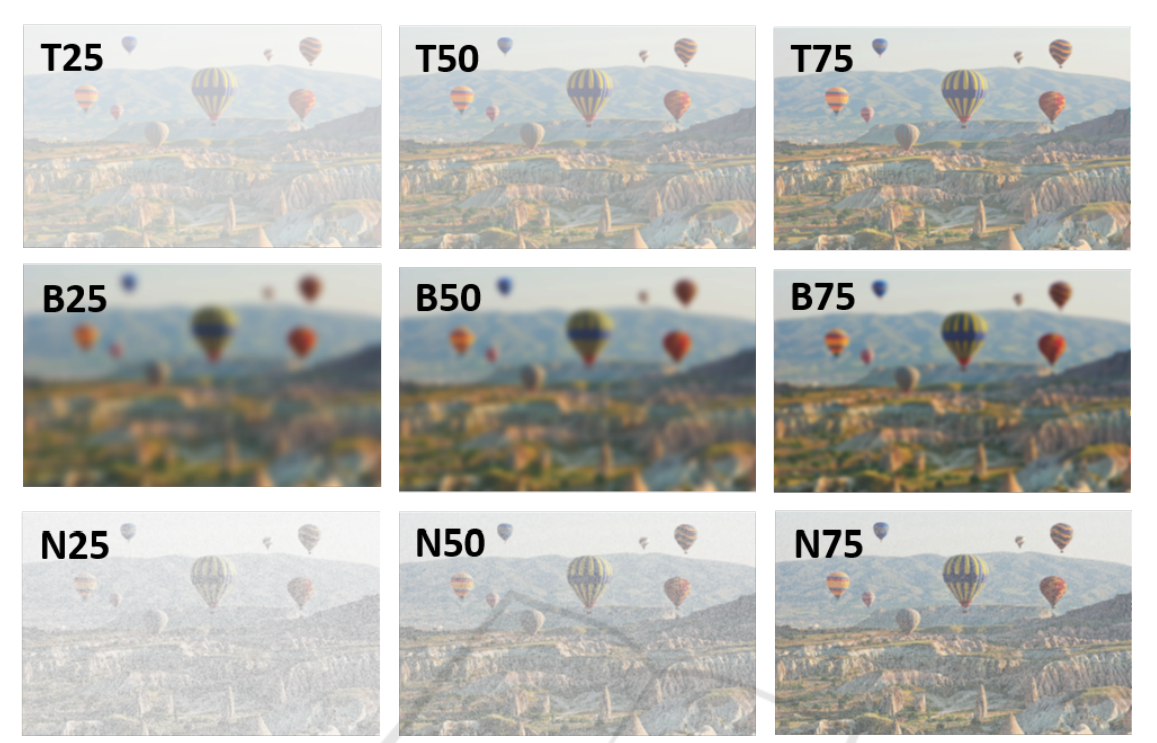
\includegraphics[width=0.9\columnwidth]{transparency-blur-noise} 
    \caption{Effetti applicati all'immagine per rendere il rischio del 25\%, 50\% e 75\%. T, B e N sono, rispettivamente, l'effetto della trasparenza, sfocatura e rumore}
\end{figure}

È stato strutturato un questionario online proposto poi a un certo numero di studenti universitari e conoscenti, i quali hanno aderito spontaneamente e senza alcun incentivo. I partecipanti avevano come compito quello di associare due delle 6 VV (2VV scelte casualmente per ogni effetto visivo) in due compiti di difficoltà crescente. Per tutti e due i compiti, è stato somministrato un set di riferimento a tre VV che indicavano un valore del 0\%, 50\% e 100\%, rispettivamente.\\
Il primo compito è stato indicato come compito di accuratezza visiva (RA): gli studenti dovevano indicare se la VV rappresentava un valore chiaramente più alto, forse più alto forse più basso o decisamente più basso del 50\% (la soglia per decisioni puramente casuali).\\
Il secondo compito chiedeva di indicare l'esatto valore di probabilità sottostante che la VV esprimeva utilizzando una barra scorrevole con un intervallo da 0 a 100. Questo compito è stato definito come compito di accuratezza assoluta (AA).\\
Ogni partecipante doveva quindi eseguire due compiti RA e due compiti AA per ciascun effetto, per un totale di 12 compiti. Per i compiti RA sono state create due misure di accuratezza, o di efficacia delle VV: il tasso di risposte adeguatamente accurate (accuratezza adeguata); e il tasso di risposte approssimativamente accurate (accuratezza approssimativa).\\
L'accuratezza adeguata è stata ulteriormente specificata diversamente per i diversi valori percentuali: il rapporto tra il numero totale di risposte e il numero dei partecipanti che hanno risposto chiaramente più alto, forse più alto, forse più basso e chiaramente più basso, rispettivamente, per le VV al 90\%, 60\%, 40\% e 10\%, e qualsiasi tipo di attributo più alto del 50\% (e rispettivamente, più basso del 50\%) per le VV al 75\% (e 25\%).
Per le ultime due VV non è stata definita l'accuratezza approssimativa, che è stata definita per le VV al 90\%, 60\% (e 40\% e 10\%) in termini del numero di risposte più alte del 50\% (e rispettivamente, più basse del 50\%).
Si ipotizzavano due possibili fonti di bias che avrebbero potuto influenzare l' analisi:
\begin{itemize}
\item l'ordine delle domande (bias di ordine);
\item il valore della percentuale mostrata (ovvero, bias di campionamento).
\end{itemize}

Per ridurre il primo tipo di bias, il questionario online è stato implementato in modo che la presentazione dei 3 effetti diversi ai partecipanti fosse random, cioè in ordine casuale.
Nel corso dello studio sono stati coinvolti più di 100 partecipanti di età compresa tra 19 e 30 anni, tutti studenti universitari. Dopo aver escluso i partecipanti che non avevano completato il questionario, il campione finale è stato di 88 utenti. Ogni combinazione di effetto visivo, tipo di compito e valore percentuale è stata completata tra 25 e 32 volte.\\
Lo scopo dello studio era capire se le rappresentazioni visive (VV) fossero un mezzo efficace per trasmettere probabilità e rischio. L'accuratezza delle risposte è stata valutata attraverso test statistici, misurata in termini di accuratezza adeguata e approssimativa per i compiti di RA, e in termini di differenza tra il valore stimato e quello reale per i compiti di AA.\\
Sono stati utilizzati intervalli di confidenza e test di ipotesi non parametrici (test del Chi-quadrato e test Binomiale) per garantire che le conclusioni fossero più conservative e affidabili. Tuttavia, non sono state rilevate differenze significative tra i tre metodi di creazione delle VVs, tranne nel caso del livello al 40\%, dove l'effetto Trasparenza è risultato significativamente più efficace dell'effetto Rumore.\\
L'analisi esplorativa ha mostrato che i valori percentuali piccoli erano sovrastimati, mentre quelli alti erano sottostimati. Test non parametrici (Mann Whitney U) hanno confermato questa tendenza, con risultati significativi per i livelli di rischio al 10\% e al 25\%. Superato il 50\%, l'effetto si invertiva, mostrando una sottostima dei valori reali. I risultati dettagliati sono riportati nelle figure dello studio.\\

Le conclusioni sono che visualizzazioni vaghe sono utili per rappresentare la probabilità e se un metodo di visualizzazione vaga è migliore tra quelle studiate. Tutti e tre gli effetti  comunicano efficacemente l'incertezza se i rischi sono superiori o inferiori al caso delle percentuali (cioè, una percentuale inferiore al 50\% è correttamente percepita così, così come quelle superiori al 50\%). In particolare le visualizzazioni vaghe sono uno strumento valido per comunicare valori intermedi, mentre è stata registrata una regressione alla media quando vengono mostrati valori estremi.
Infine, non è stato individuato un metodo migliore di altri. Gli studiosi contano di effettuare altri esperimenti in ambienti controllati e reali per verificare se le decisioni prese dai medici sono diverse quando la previsione del rischio è rappresentata con quantità evidenti, o mediante una visualizzazione vaga. Si conta anche di misurare la soddisfazione dei medici.\\

Un altro studio interessante che utilizza le visualizzazoini vaghe è lo studio "Comparative Assessment of Two Data Visualizations to Communicate Medical Test Results Online"\footcite{womak:comparative-assesment}, dove si prendono in esame test diagnostici basati su biomarcatori, cioè indicatori di una specifica condizione, nella fattispecie l'infezione da SARS-CoV-2, causa di COVID-19.\\

Ogni test diagnostico, sia esso basato su imaging, carica virale o presenza di antigeni, è associato a un certo margine di errore, ma razionalmente tendiamo a considerare l'esito del test solo in termini di sì/no, evitando di valutare la probabilità di avere o non avere una specifica condizione. Utilizzando gli
strumenti di supporto decisionale basati su ML, l'elemento probabilistico può essere reso visibile e quindi esplicitato, ad esempio riportando i punteggi di probabilità o rappresentandoli in un qualche modo: in questo studio i ricercatori ritengono che questo possa aiutare gli utenti ad interpretare al meglio l'output della
macchina. In pratica l'incertezza intrinseca di questi modelli può costituire un plus nel processo decisionale, ad esempio per scegliere se sottoporsi ad un ulteriore esame o per prediligere una terapia.\\

Tale studio ha quindi lo scopo di scegliere la migliore visualizzazione dei dati da presentare agli utenti relativamente ad un test ematologico per rilevare le infezioni da COVID-19, mediante il Conteggio Ematologico Completo, utilizzando un modello di ML. Questo modello è stato convalidato nella letteratura di riferimento e poi incorporato in uno strumento basato sul Web.\\
Sono state confrontate due visualizzazioni progettate secondo i principi delle visualizzazioni vaghe:
le stime incerte sono rappresentate evitando volutamente l'utilizzo dei simboli, cioè numeri e
rappresentazioni metriche, come estensioni della lunghezza e angoli. Secondo le caratteristiche
delle visualizzazioni vaghe, le quantità probabilistiche sono presentate come indizi visivi, i quali
sono difficili da interpretare in termini razionali, cioè sono difficili da associare a valori numerici. Si
utilizzano specificamente tonalità di colore o gradienti di saturazione e luminosità. Questa
modalità è voluta e mira a comunicare ai lettori un senso di incertezza e vaghezza per far sì che i
lettori comprendano effettivamente le stime visualizzate, come rischi, probabilità, dispersione. È
evidente che le visualizzazioni vaghe richiedono una attenzione aggiuntiva.\\

Le due visualizzazioni citate sono state ideate durante due sessioni di progettazione in cui sono
stati coinvolti sia gli autori di questo articolo sia i clinici che hanno sviluppato il modello statistico. I
clinici sono stati adeguatamente edotti circa le caratteristiche delle visualizzazioni vaghe e sono
stati invitati a co-progettare due visualizzazioni: una visualizzazione destinata a colleghi esperti
nell'interpretare i test di laboratorio, e una più semplice che potesse essere più
familiare ai pazienti testati.\\
Le visualizzazioni risultanti si basavano su metafore diverse: la prima visualizzazione si basava sul comune \gls{test-del-tornasole} e sulla metafora della bolla livello; la seconda visualizzazione dei dati adottava la metafora del bastoncino di test, utilizzata, ad esempio, nei test di gravidanza, e quindi familiare al pubblico in generale.
Lo studio è stato concepito per capire:\\
\begin{enumerate}
    \item se la metafora del bastoncino di test fosse adeguata in caso di una risposta sensibile e delicata
    come quella relativa alla positività al COVID-19, o, come osservato in alcuni studi, finisse per
    confondere troppo spesso le persone comuni
    \item se una visualizzazione dei dati più tecnica, quella progettata per gli operatori sanitari, potesse
    essere comprensibile anche al pubblico comune.
\end{enumerate}
Nella visualizzazione a bolla livello, il risultato del test è presentato attraverso la posizione di una bolla circolare all'interno di una barra a tre colori (simile al tornasole). Si valuta quindi la sua maggiore o minore vicinanza a uno degli estremi della barra per indicare una condizione COVID-19-positiva o negativa (rispettivamente all'estremo rosso più a sinistra e all'estremo blu più a destra). I risultati incerti, cioè quelli a bassa affidabilità, sono caratterizzati da una sostanziale equidistanza della bolla dagli estremi, corrispondente ad un posizionamento nella zona grigia centrale della barra tornasole. L'incertezza è anche resa evidente dalla dimensione della bolla: più grande è la bolla, maggiore è l'intervallo di confidenza della stima della probabilità.\\

\begin{figure}[!ht] 
    \centering 
    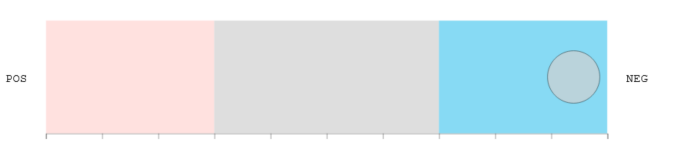
\includegraphics[width=0.9\columnwidth]{metafora-bolla} 
    \caption{Natura dell'incertezza}
\end{figure}

\begin{figure}[!ht] 
    \centering 
    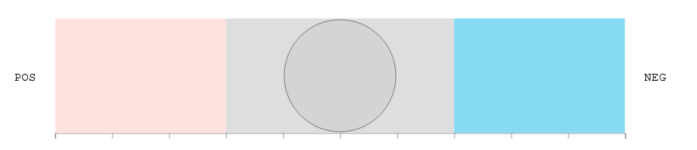
\includegraphics[width=0.9\columnwidth]{metafora-bolla-2} 
    \caption{Natura dell'incertezza}
\end{figure}

La visualizzazione del bastoncino di test fornisce le medesime informazioni visualizzate tramite la
bolla livello, ma attraverso affordance (in senso generale, favorire l'utilizzo) e segnali visivi diversi.
Nel dettaglio si vedono due fasce rosse: una per indicare l'affidabilità della risposta e indicata con
una C maiuscola ("controllo"), e una che indica il risultato del test, indicata con un segno più
singolo (+). In pratica questa visualizzazione restituisce l'output del modello in termini di opacità
della barra: più trasparenti (e meno visibili) sono la fascia + e la fascia C, minore è la probabilità
che il test sia associato a una condizione positiva e che il test sia affidabile. Un
test quasi certamente negativo è quindi reso da un bastoncino in cui è chiaramente visibile solo la
barra C,mentre un test non valido è rappresentato da un bastoncino in cui nessuna fascia rossa è
visibile.